\section*{Introduction}


The adoption of the Precautionary Approach to fisheries management \citep[PA,][]{garcia1996precautionary} requires a formal consideration of uncertainty. This had led to the use of Management Strategy Evaluation (MSE) is to develop robust advice that can still meet management objectives despite uncertainty. When conducting MSE Operating Models (OMs) are used to represent alternative hypotheses about the dynamics of the system. The most common procedure when is to fit to the available data on the basis of some statistical criterion, such as a Maximum Likelihood. The aim of this conditioning process is to reject OMs that do not fit the data satisfactorily, and are inconsistent with the actual dynamics.  

 There has been a trend when conducting MSE to use integrated assessment models for conditioning, as this allows different sources of data to be combined into a single model by a joint likelihood  \citep[e.g.][]{doubleday1976least,fournier1982general,maunder2013review}, as this allows scientists seek to use the models to capture all knowledge about stock size and productivity \citep{hilborn2003state}. Problems remain, however, including a lack of information on spatial and temporal processes that may affect stationarity,  density dependence, and conflicts between datasets. Misspecification of key parameters or assumptions in integrated stock assessment models can strongly impact the estimates of quantities of management interest, such as stock depletion and biomass at maximum sustainable yield \citep{mangel2013perspective}. Therefore, the impact of uncertainty about resource dynamics is commonly evaluated by the use of a grid-based design that considering alternative model structure, datasets and parameters \citep{sharma2020mse}. 
 
 Integrated models are commonly used to conditioning Operating Models (OMs) as part of Management Strategy Evaluation (MSE). This involves fitting an OM of the resource dynamics to the available data on the basis of some statistical criterion, such as a Maximum Likelihood.  The aim of conditioning is to reject OMs that do not fit the data satisfactorily, and are consequently inconsistent with the actual situation observed and therefore implausible. Therefore, when conditioning OMs the intention is not to find a "best assessment" but a limited set of OMs with high plausibility, which include the most important uncertainties in the model structure, parameters, and data. Plausibility may be estimated formally based on some statistical approach, or specified based on expert judgement, and can be used to weight performance statistics when integrating over results for different scenarios (OMs). The methods developed in the cookbook can be used to do this. 
 
 To date, however, little effort has gone into weighting of the different models, e.g. based on ensemble modelling. Advice, however, depends on the weights given to the different models when post processing, and critically the original choice of models. Therefore questions that need to be answered in the conditioning are does the model presents a good fit to the data and is it able to predict the response to fishing \citep{carvalho2020cookbook}. We therefore develop a schema for weighting and potential rejection of stock assessment model scenarios, and compare different metrics to simple skill-based weighting (SW).
 

\section*{Material and Methods}

An Operating Model for the albacore tuna (\textit{Thunnus alalunga}) fishery and stock in the Indian Ocean has been developed by the Indian Ocean Tuna Commission (IOTC) to evaluate the performance of alternative Management Procedures (MPs).  The Operating Model (OM) was conditioned using stock synthesis \citep[SS3][]{MethotW2013} based on current best knowledge and data \citep{ptmt2014}. Datasets include records of catches and landings, indices of abundance based on catch per unit (CPUE), and  length and ages compositions from samples. Reformulating model structure, however, is time consuming and so scenarios were based on the choice of parameters for which there is insufficient information in the data to estimate and data weighting. 

\subsection*{Material}

The assesssment partitions the Indian Ocean into four regions, divided latitudinally along the 25$^{\circ}$S parallel and longitudinally along the 75$^{\circ}$E meridian. Aggregated catches (in numbers of fish) for the Japanese and Taiwanese LL fleets, for the 1950-2014 period, are shown. From \citep{LangleyH2016}, figure \ref{fig:map} show the distribution of catches across the areas defined in the assessment. The model includes a total of 11 fisheries, including in this case an aggregaqted Longline fishery for each of the four regions. For a detailed explanation of the data and fleets included in each of these fisheries, please refer to \citep{LangleyH2016}. A new set of standardized CPUE indices has been derived using generalized linear models (GLM) operational from longline catch and effort data provided by Japan, Korea and Taiwan, China. \citep{HoyleKL2016}. The operating model conditioning used the same series as the final runs of the stock assessment \citep{LangleyH2016}, a combined industrial longline series, on each of the four areas, and restricted to the 1979-2014 period (Figure \ref{fig:cpues}). Of these four areas, area 3 is considered to represent the core of the distribution of the stock. The management procedures tested make use of a single CPUE, taken to be that corresponding to area 3.

The distribution of catches by assessment areas are shown in are shown in figure \ref{fig:map}.
   
Fisheries data is in general less informative that would be ideal when it comes to estimating a large number of model parameters, which are often correlated. In the case of the Indian Ocean albacore stock, a number of reasons are limiting our ability to obtain reliable model fits. Problems exists with the data completeness and quality \citep{IOTC2016WPTmT0607}, not limited to but including total catch statistics, length distribution in catches, and biological information. We also depend on our ability to produce sensible indices of changes in abundance in the stock based only on Catch-per-unit-effort data from commercial fleets, where issues of targeting, operating and others are all known to influence the relationship between stock abundance and CPUE, despite recent work on standardization of the longline CPUE series for this stock \citep{oyleKL2016}.

The seven factors currently considered in the structural uncertainty grid for the albacore OM are shown in  table \ref{tab:om})

A common unknown in most stock assessment models, the base case considered in the stock assessment session was supplemented with alternative values of higher and lower M for either all ages, or different for juveniles (ages 0 to 4) and adults (age 5 or older), for a total of five possibilities. Two values were considered for the true variability of recruitment in the population, 0.4 and 0.6. Three values for the steepness (h) of the stock-recruitment relationship are being used: 0.7, 0.8, and 0.9. The Beverton and Holt stock-recruit model implemented. Four values for the coefficient of variation in the CPUE series were included: 0.2, 0.3, 0.4 and 0.5. Three values were used for the relative weight of length sampling data in the total likelihood, through changes in the effective sampling size parameter, of 20, 50 and 100. This alters the relative weighting of length samples and CPUE series in informing the model about stock dynamics and the effects of fishing at length. Two scenarios were considered for the effective catchability of the CPUE fleet. On the first one it was assumed that the fleet had not improved its ability to fish for albacore over time, or that any increase had been captured by the CPUE standardization process. An alternative scenario considered a 2.5\% increase in catchability by correcting the CPUE index to reflect this.  Two possible functional forms for the selectivity of the CPUE LL fleet were considered: a logistic function (Log), where selectivity stays at the maximum level, or double normal (DoNorm), where selectivity drops at some point in the age range.


\subsection*{Methods}

The performance of multimodel ensembles depends on the weights given to the different models in postprocessing. Although still common practice, equal weighting of all models in a grid or ensemble may result in biased advice if too much weight is assigned to models that fit the data poorly or have low have poor prediction skill \citep{kell2020yft}.

We therefore explore a number of different potential weighting schema, and methods for selecting and rejecting OM scenarios, and compare equal weighting (EW), with simple skill-based weighting (SW) \citep{casanova2009weighting}.

\subsubsection*{Weighting}

%Considering alternative structures and datasets means that it difficult to select models using metrics such as AIC. Therefore retrospective analysis is commonly used to evaluate the stability of stock assessment estimates of model estimates such as stock biomass and exploitation level. Stability is measured using Mohn's $\rho$ a measure of bias. Shrinking estimates of stock status in the last year to the recent mean can help reduce Mohn's $\rho$. Shrinkage, in statistics, however, is used to reduce mean squared error (MSE), at the expense of bias. The use of model based quantities, however, means that bias can not be quantified, and may result in forecasts having little prediction skill. We therefore extend retrospective analyses to include prediction. 

\begin{description}
\item[Expert] Stakeholder concerns and expert opinion, assigned “a-priori”, without consideration of model fit.
 \begin{itemize}
    \item How were scenarios selected?, e.g. through an elicitation process \citep{leach2014identification}?
\end{itemize}
\item[Convergence] Model convergence criteria of the estimation algorithm. 
\begin{itemize}
    \item max gradient? This is normally achieved by jittering, however this is difficult to do in this case where 1440 grids are run. Therefore we explore what factors result in poor convergence.
\end{itemize}
\item[Diagnostics] Reliability of the model based on residual diagnostics
 \begin{itemize}
    \item Use runs tests to check for randomness in the residuals 
\end{itemize}
 \item[Fit] The fit of the model to the data
 \begin{itemize}
    \item Likelihood, we do not use AIC due to problems in weighting and the fact that since the number of parameters only changes for 1 scenario the AIC and likelihoods are equivalent. Using the likelihood also allows us to look at data components.
\end{itemize}
\item[Plausible parameters] The plausibility of the estimates of the parameters representing the dynamics
 \begin{itemize}
    \item  $r$, $K$ and $p$, i.e. production functions
\end{itemize}
\item[Plausible results] Time series dynamics and process error.
\begin{itemize}
    \item ACF of biomass
    \item clockwise SP
    \item var(SP)
\end{itemize}
\item[Stability] Retrospective
https://www.overleaf.com/project/5f06c2b7d4ece70001d5c362\begin{itemize}
    \item traditional Mohn's $\rho$
\end{itemize}
\item[Prediction Skill] Model outputs
 \begin{itemize}
    \item 3 year ahead Mohn's $\rho$ 
\end{itemize}
\item[Prediction Skill] Model free
\begin{itemize}
    \item MASE for CPUE
\end{itemize}
\end{description}

\subsubsection*{Runs Test}

Analysis of residuals is a common way to determine a model’s goodness-of-fit \citep{Cox1968general}, since  non-random patterns in the residuals may indicate model misspecification, serial correlation in sampling/observation error, or heteroscedasticity. 

When inspecting residuals, however, there is a danger of hypothesis fishing and if multiple true hypotheses are tested it is likely that some of them will be rejected. Therefore it is valuable to reserve part of the data for validation, so that a pattern’s significance is not tested on the same data set which suggested the pattern.


If the process of interest shows only random variation, the data points will be randomly distributed around the median. Random meaning that we cannot know if the next data point will fall above or below the median, but that the probability of each event is 50\%, and that the data points are independent. Independence means that the position of one data point does not influence the position of the next data point, that is, data are not auto-correlated. If the process shifts, these conditions are no longer true and patterns of non-random variation may be detected by statistical tests. Various statistics exist to evaluate residuals and nonparametric tests for randomness in a time-series include: the runs test, the sign test, the runs up and down test, the Mann-Kendall test, and Bartel’s rank test.

Non-random variation may present itself in several ways. If the process centre is shifting due to improvement or degradation we may observe unusually long runs of consecutive data points on the same side of the median or that the graph crosses the median unusually few times. The length of the longest run and the number of crossings in a random process are predictable within limits and depend on the total number of data points in the run chart \citep{anhoj2015diagnostic}.

A shift signal is present if any run of consecutive data points on the same side of the median is longer than the prediction limit, round(log2(n) + 3). Data points that fall on the median do not count, they do neither break nor contribute to the run \cite{schilling2012surprising}. A crossings signal is present if the number of times the graph crosses the median is smaller than the prediction limit, qbinom(0.05, n - 1, 0.5) \citep{chen2010impacts}. n is the number of useful data points, that is, data points that do not fall on the median. The shift and the crossings signals are based on a false positive signal rate around 5\% and have proven useful in practice.
\input{Hindcast}
\subsubsection*{Generating delta-MVLN Kobe posteriors}

Generate Kobe posteriors from a MVLN distribution requires the means and the variance-covariance matrix (VCM) of $log(SSB/SSB_{MSY})$ and $log(F/F_{MSY})$. Let $u = SSB/SSB_{MSY}$ and $v = F/F_{MSY}$  and $x = log(u)$ and $y = log(v)$ , then the $VCM$ has the form:
    			
\begin{equation}
VCM_{x,y} =
\begin{pmatrix}
\sigma^2_x & cov_{x,y}  \\
cov_{x,y} & \sigma^2_y
\end{pmatrix}
\end{equation*}

where  is the variance of x,  is the covariance of y and  is the covariance of x and y.  The quantities that can be directly extracted from Stock Synthesis are: (1) MLEs, asymptotic standard errors (SE) and correlation of $SSB/SSB_{MSY}$  and $F/F_{MSY}$. 
The construction of the  therefore requires to conduct a few normal to lognormal transformations. First, we approximate  and  as:

\begin{equation}
\sigma^2_x = \disp log\left(1+\left(\frac{SE_u}{u}\right)^2\right)  
\quad 
\end{equation}

and

\begin{equation}
\sigma^2_x = \disp log\left(1+\left(\frac{SE_v}{v}\right)^2\right)  
\quad 
\end{equation}

where  and  is the asymptotic standard error estimate for $u = SSB/SSB_{MSY}$ and $v = F/F_{MSY}$. Second, the covariance of x and y can then be approximated on log-scale by:

\begin{equation}
COV_{x,y} = \disp log \right{1+ \rho_{u,v} \sqrt{\sigma^2_x\sigma^2_y}\right \quad 
\end{equation}

where  donates the correlation of u and v.
To generate the desired KPD for $SSB/SSB_{MSY}$  and $F/F_{MSY}$, we use a multivariate random generator, available in the R package ‘mvtnorm’, to obtain a large number (nsim = 10,000) of x and y pairs, such that

\begin{equation}
kobe_{x,y} = \disp MVN{\mu_{x,y},VCM_{x,y}) 
\quad 
\end{equation}

where  is the vector of the MLEs x and y. The joint MVLN distribution of $-SSB/SSB_{MSY}$  and $-F/F_{MSY}$ is then obtained as the exponential of $kone_{x,y}$.



There are a variety of frequentist model-weighting strategies ranging from giving all models in S a weight related to the AIC (Akaike information criterion) or BIC (Bayesian information criterion) of each model, to an interpolation between two extreme cases. We present an AIC-based weighting strategy called smooth AIC weights that was first presented by Buckland et al. (1997). In smooth AIC weighting, the weights are given by:  
wM=exp(−(1/2)AICM)∑M′∈Sexp(−(1/2)AICM′).
(6)

It is suggested to subtract the minimum AIC from each model AIC to avoid numerical issues when taking exponents.

%In age-structured models, there is an implicit production function, and changes in productivity can occur due to process error modelled as variability in recruitment and selection pattern. In the biomass-dynamic models with an explicit production function, process error is modelled explicitly.

In age-structured models, density dependence is mainly accounted for by the stock-recruitment relationship. Cury et al. (2014), however, showed that in most cases the stock-recruitment relationship used to estimate productivity and determine reference points, has poor estimation/predictive power and the environment has a larger effect on productivity, a result confirmed by other studies (e.g. Szuwalski et al., 2015, 2019; Free et al., 2019), and observed 100 years ago by Hjort (1914). Whereas in ICCAT assessments growth, maturation and natural mortality are assumed not to have varied despite the significant changes in the environment and stock biomass seen.

Hilborn (2001) therefore recommended looking at patterns of change in surplus production (SP) since these may contain evidence of changes in the growth and mortality components of production, which are typically not represented in models currently used for stock assessment and management. 

Walters et al. (2008) argued that plotting of surplus production (SP) against biomass (B) should be one of the basic pieces of information presented in all stock assessments since the plots provide a check on whether there has been non-stationarity in the annual surplus production, i.e. whether similar B levels have exhibited similar SP at different historical times. This is important for management as it checks whether predictions of changes in biomass (Bt+1−Bt) can be made reliably based on catch and Bt. Plots of SP v B therefore provide a summary of stock performance and include effects not necessarily included in stock assessment models.

The effects not included in the production function used to predict SP can be modelled by a process error term # t.

				$B_{t+1} = B_t − C_t + SP_t + ε_t$

Process error on biomass can account for model structural uncertainty as well as natural variability of stock biomass due to stochasticity in recruitment, natural mortality, 4growth, and maturation (Francis and Hilborn, 2011; Meyer and Millar, 1999; Thorson et al., 2015).

We, therefore, examine the relationships between surplus production and biomass . To do this, we estimate annual surplus production as the change in stock size plus catch (i.e. $B_t – B_{t+1} + C_t$). We then plot the resulting time series of S and B to identify patterns of variation in S. The process error was then sampled from SS3 stock trajectories as the difference between the deterministic expectation of biomass and its stochastic realisation, such that:

				$ε_t = SB_{t+1} - (SB_t + SP_t − C_t)$ 



\newpage
\section*{Results}

\begin{itemize}
   \item Time series of catch, and spawning stock biomass and fishing mortality relative to $MSY$ target reference points are shown in figure \ref{fig:ts} for the base case (black line) the main effects. Catches have increased since the 1950s, and in the last two decades have varied just above $MSY$. This has resulted in an increase in $F$ and a decrease in $SSB$, although the stock is assessed to be above $SSB/B{MSY}$ and in only a few cases is $F$ above $F_{MSY}$.  

   \item The production functions from which the $MSY$ reference points are derived are shown in figure \ref{fig:pf}. There are two main features a change in the shape of the production function with steepness, and an increase in scale as the natural mortality of adults increases or the length composition effective sample size decreases. The increase in adult M, the shape of the production function, results in the stock becoming more robust to exploitation, since to explain the catches the stock most be more productive, as seen by the increase of the slope at the origin, and hence population growth rate ($r$)  

   \item Kobe phase plots (figure \ref{fig:kobe}) showing $SSB/B_{MSY}$ and $F/F_MSY$ in the terminal year are shown for the main effects with estimation error approximated using a multivariate log-normal, (cyan points denote the median) in figure \ref{fig:kobe-main}, and the base case is compared to the full grid in figure \ref{fig:kobe-bg}. The base case only gives a X\% chance of being in the green quadrant ($SSB \gt SSB_{MSY}$ and $F \le F_{MSY}$) when estimation error is considered. Although only 1 main effects (M0202?) is in the red quadrant, X\% are in the red quadrant when estimation error is considered, while when model error is considered this increases to Y\%. 
   
   \item Summary of Mohn's $\rho$ for the for the 1440 assessment models in the Indian Ocean albacore tuna grid, with main effects indicated by the vertical lines (Figure \ref{fig:mohn}). Four of the main effects fail the Mohn's $\rho$ test. There appears to be bi-modality with one mode centred on 0, i.e. some scenarios perform very well compared to the main effect and base case.
   
   \item This shows that uncertainty is underestimated if only estimation error is considered. This implies over-fitting and a subsequent reduction in variance at the expense of bias. Figure \ref{fig:runs} therefore compares the runs tests based on the model residuals to the prediction residuals for the entire grid. The number of crossings (figure \ref{fig:runs-cross}) and the length of the longest run (figure \ref{fig:runs-long} and the MASE (figure \ref{fig:mase}). Most of the scenarios and indices pass the crossings test, while performance for the length of the longest run is poorer. Indices 2 and 3 perform best. The value of Mohn's $\rho$ does not appear to have an impact. 
   
   \item The results for MASE from the model-free hindcast are different from the runs tests, in that Mohn's $\rho$ does appera to have an effect, i.e. a scenario and index has a value of $MASE \gt 1$ it also tends to have lower prediction skill.  While the relative performance of indices 2 and 3 is similar to the runs tests, index 4 now has good performance.
   
   \item The p-values by scenarios for MASE and the runs test are compared to Mohn's $\rho$ in figure \ref{fig:wts}. These show that in the sceanrios with good prediction skill indices perform better, based on MASE. The runs test does not appear to be an indicator of prediction skill, potentially due to overfitting. 

   \item A Regression tree identifying factors that influence Mohn's $\rho$ for the 1440 assessment models is shown in Figure \ref{fig:tree}. This also shows the time series of SSB (\ref{fig:tree-b}), production functions (\ref{fig:tree-pf}), and time series of surplus production (\ref{fig:tree-sp}). The first split is on natural mortality of the adults, if this is equal to 0.4 then the Mohn's $\rho$ test is failed, otherwise it is passed. These, as seen above have lower estimated values of $B_{MSY}$ and $MSY$. The two exceptions are for M=0.3 and CPUE = 0.2 \& 0.3 when it fails, and M=0.4 and CPUE=0.5 \& ESS = 100 when it passes. In other word the biggest impact on prediction skill is M, since high M results in a large productive stock which is not supported by the hindcast. High M is only plausible if you ignore the CPUE and fit to the length data. 
   
  \item Weighted phase plots are presented in figure \ref{fig:phase-wt} for equal, simple skill based, and AIC weighting. These are for targets (Kobe \ref{fig:kobe-wt}) and limits (Majuro \ref{fig:majuro-wt}). 

  \item Figure \ref{ref:grid} summarises a variety of summary metrics by adult M and steepness for Mohn's $\rho$. $SSB/B_{MSY}$ (\ref{fig:grid-bmsy}), $B_{lim}$ (\ref{fig:grid-blim}), $F/F_{MSY}$ (\ref{fig:grid-fmsy}), $r$ (\ref{fig:grid-r}), $K$, (\ref{fig:grid-k}), $p$, (\ref{fig:grid-p}), $sd(sp)$, (\ref{fig:grid-sp}), and Population doubling time (\ref{fig:grid-dt}). There is some modality due to catchability, particulary in current biomass status and $K$.  Again the biggest impact is adult M. 

\end{itemize}




\clearpage
\newpage
\newpage
\section*{Discussion}


When developing metrics as in any indicator, the total number should be minimised, complementary and non-redundant (Shin et al. 2010; Kershner et al. 2011). They should also be robust proxies for relevant attributes, and need to be screened using appropriate selection criteria \cite{kell2020roc}. To be effective a metric should be robust, so that it still functions despite uncertainty \parencite{radatz1990ieee, zhou1996robust}. To be robust an metric should be both reliable and stable. A metric has high reliability if despite uncertainty it provides an accurate result, and it is stable if despite random error, similar results are produced across multiple trials. 

\begin{itemize}
    \item The aim of this work was to evaluate the use of full factorial designs for representing uncertainty in stock assessment. In particular to identify the assumptions that impact the perception of stock dynamics and status, and develop tools for weighting or rejecting stock assessment scenarios.
  
    %\item The Indian Ocean Albacore MSE used Stock Synthesis to develop scenarios based on parameters that are difficult to estimate (i.e. M, steepness, and selectivity) and the relative weightings of the indices of abundance and the length data. The choice of OMs is important as the \textit{best} Management Procedure is determined by the choice of hypotheses represented by the OM. It seldom possible, however, to assign plausibility to the different scenarios, therefore the rationale for the grid design is of fundamental importance.

    %\item Need to consider the future not just the past
    
    \item The absence of retrospective patterns in model quantities such as stock biomass, is not sufficient to validate models based on model outputs, since a small RE could be achieved by a model that used no data.  Therefore conduct a hindcast.
    
    \item Can only validate models on observations and not model outputs, therefore need to conduct model free hindcasts to estimate prediction skill by comparing observations and to their model estimates, to explore bias, variability and prediction skill.
    
    \item Use the hindcast procedure to weight multi-model ensembles using simple skill-based weighting. A prediction skill score can be used to assign more weight on the better performing models as this has been found to improve forecasts \citep[e.g.][]{casanova2009weighting}. This can be done to weight estimates of current status relative to reference points, or weight operating models when conducting MSE. %Testing the approach on an actual case study first was informative as it provides the insight necessary to set up a study on synthetic data.

    %\item next step is assess prediction skill using model free hindcasting, as it allows comparisons to be made across model structures and datasets. Validation examines if a model family should be modified or extended and is complementary to model selection and hypothesis testing. In comparison model selection searches for the most suitable model within a family, whilst hypothesis testing examines if the model structure can be reduced. This is important as it allows alternative model frameworks to be compared and valiadated in a working group setting.

    %\item When conducting Management Strategy Evaluation (MSE) Operating Models (OMs) are commonly \citep{Sharma} conditioned using stock assessment models and a grid design to model structural uncertainty and data conflicts. However, there are two main characteristics of the stock dynamics i.e. the expected dynamics as represented by a production function and the nature of the times series. Therefore you could just run a limited number of scenarios that represent the different production functions an time series dynamics.

    \item \cite{fischer2020linking} showed that to develop robust management strategies the nature of the time series of the stock has to be considered. The importance of this is that trends and fluctuations in populations are determined by complex interactions between extrinsic forcing and intrinsic dynamics. For example, stochastic recruitment can induce low-frequency variability, i.e. ‘cohort resonance’, which can induce apparent trends in abundance and may be common in age-structured populations \citep[e.g.][]{bjoernstad2004trends, botsford2014cohort}. Such low-frequency fluctuations can mimic or cloak critical variation in abundance linked to environmental change, over-exploitation or other types of anthropogenic forcing. In feedback management systems the nature of the time series dynamics is likely to be more important than the equilibrium dynamics. 
    
    \item The objective of MSE is to develop a robust MP, so weighting of OM grids based on stock assessments is a waste of time. Since trends and fluctuations in populations are determined by complex interactions between extrinsic forcing and intrinsic dynamics. For example, stochastic recruitment can induce low-frequency variability, i.e. ‘cohort resonance’, which can induce apparent trends in abundance and may be common in age-structured populations \citep[e.g.][]{bjoernstad2004trends, botsford2014cohort}. Such low-frequency fluctuations can potentially mimic or cloak critical variation in abundance linked to environmental change, over-exploitation or other types of anthropogenic forcing. In feedback management systems the nature of the time series dynamics is likely to be more important than the equilibrium dynamics.

   \item Weighting give very different results wrt targets and limits, this is important, e.g. for MSC. Rather than arguing about the best weighting scheme better to develop robust MPs, that need to be tested for a range of plausible dynamics. 
   
\end{itemize} 



\section{Conclusions}

I totally agree on the automation, to ensure objectively and transparency. Its like MSE where you have to agree the OMs and the MP selection criteria in advance.

Also like MSE, I think we need a limited number of complementary but non-redundant metrics. For example are the runs tests,  RMSE and Mohn's rho telling us the same thing? So we are give a single attribute extra weight? Imagine you have a model with a biased index, i.e. a data conflict, that fails the runs and RMSE tests. When you do retrospective you are removing biased points so you will get a large absolute value for Mohn's rho. In contrast MASE for a model free quantity will hopefully be telling you something else. It would be best to recognise that data conflict at the start.

For this reason I  agree with Mark that ideally a model should pass all diagnostics but recognise that this isn't always possible. For example if a model fails to converge that could indicate data conflicts and model misspecification, that will bite you later if not fixed. For example when you start removing points example in the retrospective analysis and hindcasts.

Also while the delta-MVLN approach is useful, I would also like to use estimation error to check bias, i.e. by looking at prediction residuals.

\begin{itemize}
    \item In the stock assessment process hypotheses about states of nature are represented by alternative model structures and fixed parameters. Even with a design of 1440, as in this example, the choice of scenarios is arbitrary and the posterior distributions are often multi-modal.
    
    \item Considering alternative structures and datasets means that it difficult to select models using metrics such as AIC. Therefore retrospective analysis is commonly used to evaluate the stability of stock assessment estimates.  The use of model based quantities, however, means that bias can not be quantified, and may result in future predictions being being poor. We therefore extended retrospective analyses to include predictions. 
   
    \item The use of metrics based on prediction skill allows different data components and model to be compared in order to explore data conflicts and potential model misspecification. The accuracy and precision of predictions depend on the validity of the model, the information in the data, and how far ahead predictions are required. 
   
    \item Retrospective analysis is commonly used to evaluate the stability of stock assessment estimates of model estimates such as stock biomass and exploitation level. Stability is measured using Mohn's $\rho$ a measure of bias. 
    
    \item Shrinking estimates of stock status in the last year to the recent mean can help reduce Mohn's $\rho$. Shrinkage, in statistics, however, is used to reduce mean squared error (MSE), at the expense of bias. 
    
    \item The use of model based quantities, however, means that bias can not be quantified, and may result in future predictions being being poor. We therefore extend retrospective analyses to include prediction. 

    \item When developing the design for ensembles or OMs first it is necessary to choose a base case, the main effects and interactions. A problem is that hypotheses are likely to be confounded e.g. i) is High M and low steepness realistic? ii) relative weighting of ESS and CPUE CV; and iii) dome shaped selection or senescence. If we had used the approach proposed would our conclusions have differed? Use of feedback relaxes requirement for prediction skill, ii) helps identify series for use in OEM, iii) what if OM scenarios have different "best" indices?

    %\item For models to be valid the situation being modelled must be observable and measurable. Therefore it is only possible to validate models on observations, the next step is to use model free hindcasting.
     
    %\item In order to develop robust advice frameworks by conducting Management Strategy Evaluation Operating Models should not be condition on stock assessments alone.

    %\item Hessian not inverting might be the most interesting result! i.e.  did we start from the wrong place, is there conflict or lack of information in the data, are the parameters confounded? is our structure wrong,... We need to answer these questions before we agree the ensemble.
    
    %\item The numerical tests may have different distributions and properties making using difficult to use for weighting, i.e. RMSE is influenced by a few outliers and is not comparable across series. While MASE  has the properties of scale invariance, predictable behaviour, symmetry, interpretability and asymptotic normality. MASE is also independent of the scale of the data, so can be used to compare forecasts across data sets with different scales, and behaviour is predictable as and a value of 0.5 means that a prediction is twice as good as one with a value of 1.
    
    %\item Tests have different purposes and different consequences, so equal weighting may be hard to justify. For example, if model residuals are fine, but prediction residuals fail. The consequences are  you may have overfitted, i.e. added too many parameters possibly as a result of hypothesis fishing, and the prediction residuals are telling you that your model is invalid, and so you need to start again.
    
    %\item  Bootstrapping depends on how the weights have been assigned and how the ensemble was selected.
\end{itemize}



\newpage\clearpage
\bibliographystyle{abbrvnat}
\bibliography{references.bib}

\clearpage
\newpage

\section*{Tables}

\begin{table}[ht]
\label{tab:grid}
\caption{Operating Model Scenarios; Base Case values in bold.}  
\begin{center}
\label{tab:datasumm}
\small

\begin{tabular}{|lccc|}

\hline
Factor & {Levels (N)} & {$\prod$ N} & {Values} \\ %& {Prior} & {Weighting}\\
\hline\hline
{Natural mortality (M)& {5}}  & {  5}  & { 0202  \textbf{0303} 0404 0403 0402}    \\
{Steepness of the stock-recruitment relationship}}& {3} 	 & {15}  & { \textbf{.7}; 0.8; 0.9} \\
{Variability of recruitment (sigmaR)}& {2} 	 & { 30}  & { \textbf{0.4}; 0.6} \\
{Effective Sampling Size of the length composition data (ESS)}& {3} & { 90}  & { 20; \textbf{50}; 100} \\
{CV for fit to CPUE (cpuecv)}& {4} 	 & { 360}  & { 0.2;  \textbf{0.3}; 0.4; 0.5} \\
{Yearly increase in catchability coefficient of CPUE (llq)}& {2} 	 & {  720}  & { \textbf{0\%}; 0.25\%} \\
  {Selectivity (llsel)}& {2}}& {1440}} & { \textbf{logistic} double normal} \\
\hline

\end{tabular}
\end{center}
\end{table}

\newpage
\newpage
\section*{Figures}

\begin{figure}[ht!]\centering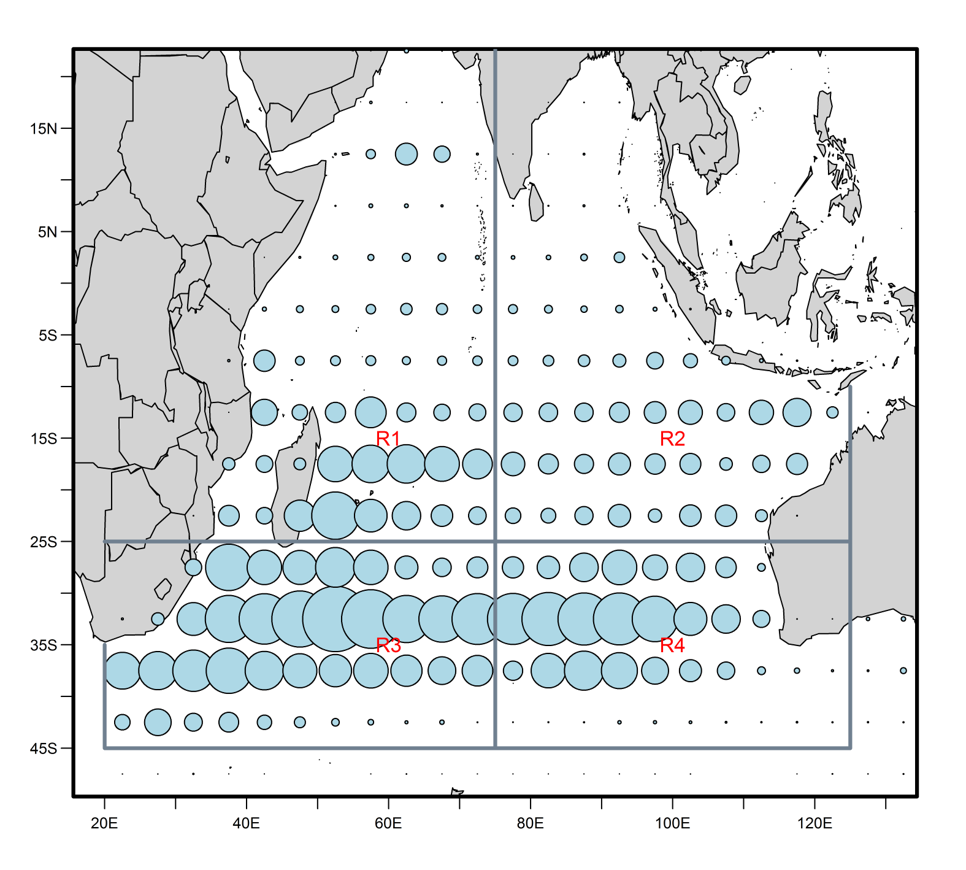
\includegraphics[width=0.75\textwidth]{figures/alb-map.png} 
\caption{Distribution of Indian Ocean albacore tuna catches by assessment areas.}
\label{fig:map}
\end{figure}

\begin{figure}[ht!]\centering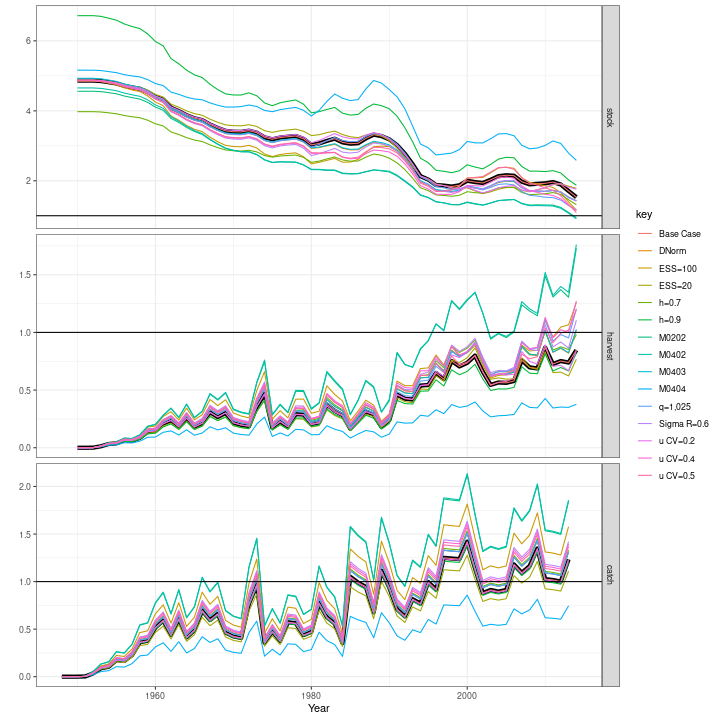
\includegraphics[width=0.75\textwidth]{figures/main-trends-1.png} \caption{Time series of spawning stock biomass and fishing mortality relative to $MSY$ target reference points for the main effects of the Indian Ocean albacore tuna assessment model grid.}
\label{fig:ts}
\end{figure}

\begin{figure}[ht!]\centering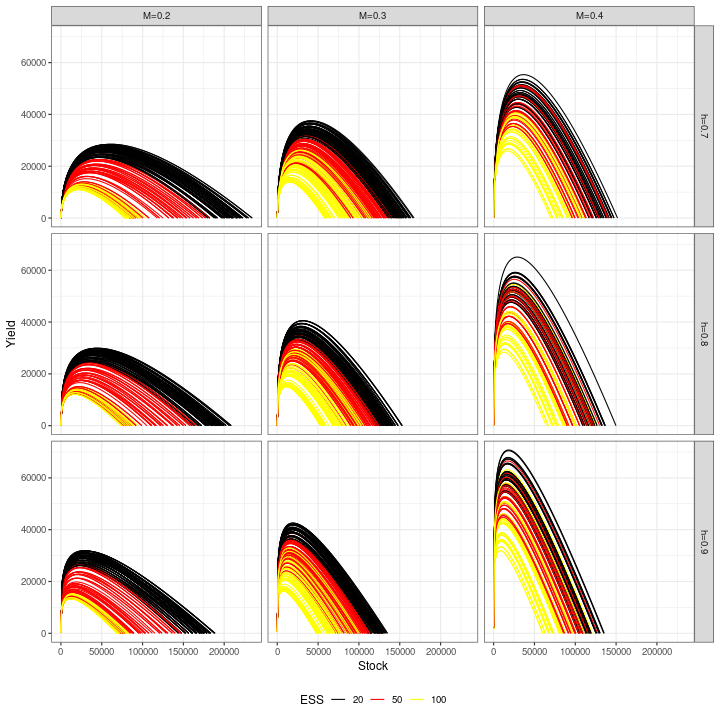
\includegraphics[width=0.75\textwidth]{figures/pf-grid-1.png} 
\caption{Production by steepness and mature natural mortality}
\label{fig:pf}       
\end{figure}

\begin{figure}
        \begin{subfigure}[b]{0.5\textwidth}
               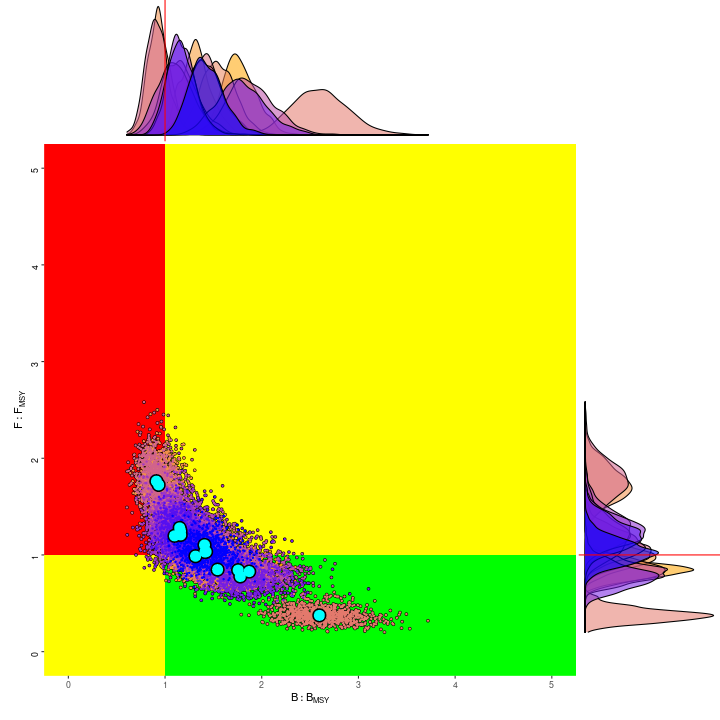
\includegraphics[width=\linewidth]{figures/kobe-main-1.png}
                \caption{Main effects with estimation error.}
                \label{fig:kobe-main}
        \end{subfigure}%
                \begin{subfigure}[b]{0.5\textwidth}
                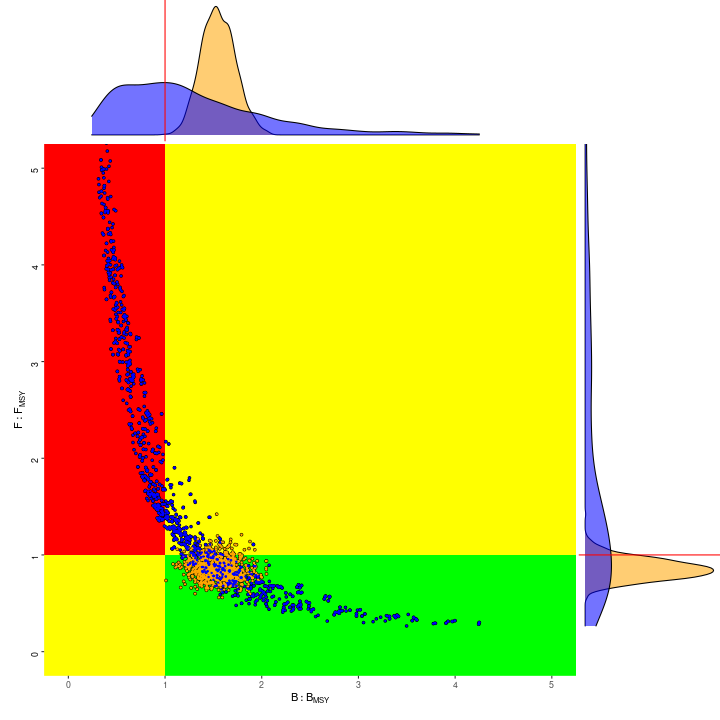
\includegraphics[width=\linewidth]{figures/kobe-bg-1.png}
                \caption{Reference case and grid with model.}
                \label{fig:kobe-bg}
        \end{subfigure}%
        \caption{Kobe phase plots showing spawning biomass ($B$) and fishing mortality ($F$) relative to $MSY$ target reference points. Within model uncertainty was approximating using multivariate log-normal distribution derived from Hessian matrix (MVLN) with cyan points denoting the median}\label{fig:kobe}
\end{figure}

\clearpage
\newpage
\begin{figure}[ht!]\centering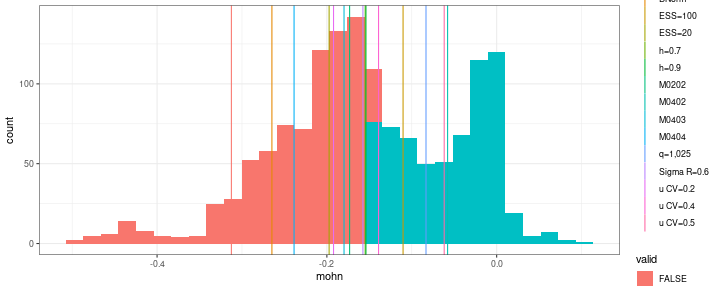
\includegraphics[width=0.75\textwidth]{figures/mohn3-1.png}  \caption{Summary of Mohn's $\rho$ for the for the 1440 assessment models in the Indian Ocean albacore tuna grid, with main effects indicated by the vertical lines.} 
\label{fig:mohn}       
\end{figure}

\begin{figure}
    \begin{subfigure}[a]{0.35\textwidth}
    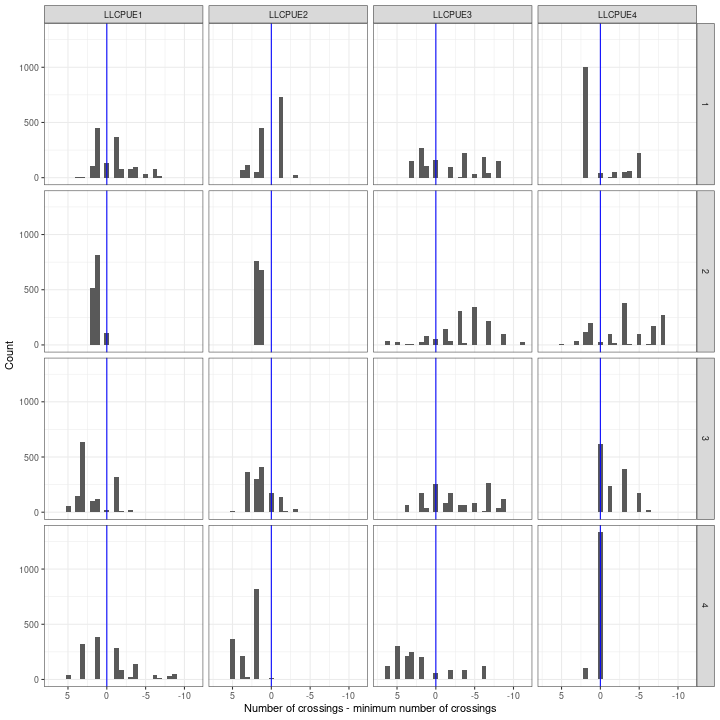
\includegraphics[width=\linewidth]{figures/run-cross-1.png}
    \caption{Number of crossings - minimum expected number of crossings; note reversed x-axis.}
    \label{fig:runs-cross} 
    \end{subfigure}%
    \begin{subfigure}[b]{0.35\textwidth}
    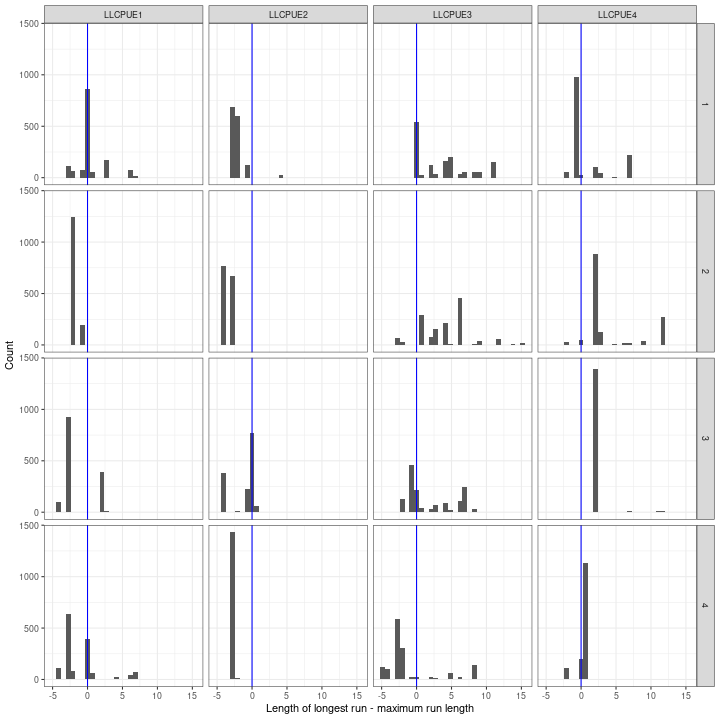
\includegraphics[width=\linewidth]{figures/run-long-1.png}
    \caption{Longest run - maximum expected run length.}
    \label{fig:runs-long}
    \end{subfigure}%
    \begin{subfigure}[c]{0.35\textwidth}
    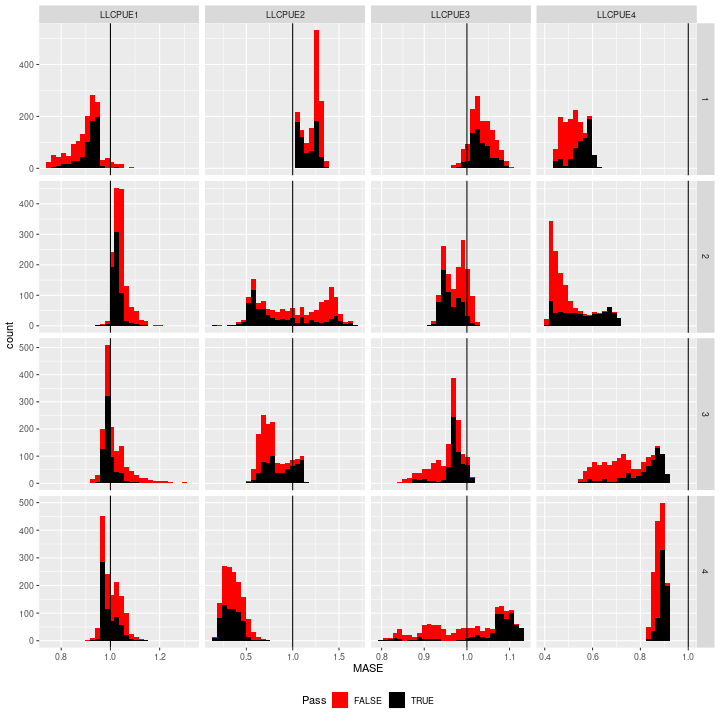
\includegraphics[width=\linewidth]{figures/mase-1.png}
    \caption{MASE.}
    \label{fig:mase}
    \end{subfigure}%
 
\caption{}\label{fig:runs}
\end{figure}


%\begin{figure}[ht!]\centering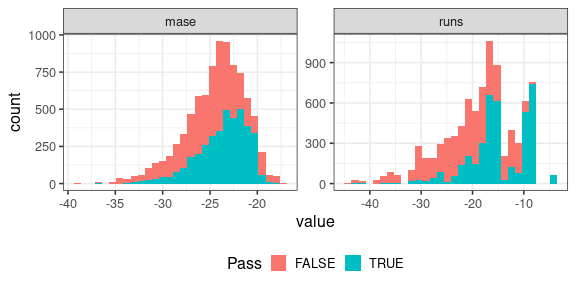
\includegraphics[width=0.75\textwidth]{figures/cf-1.png} \caption{Summary of weighting diagnostics.}\label{fig:wts} \end{figure}

\begin{figure}[ht!]\centering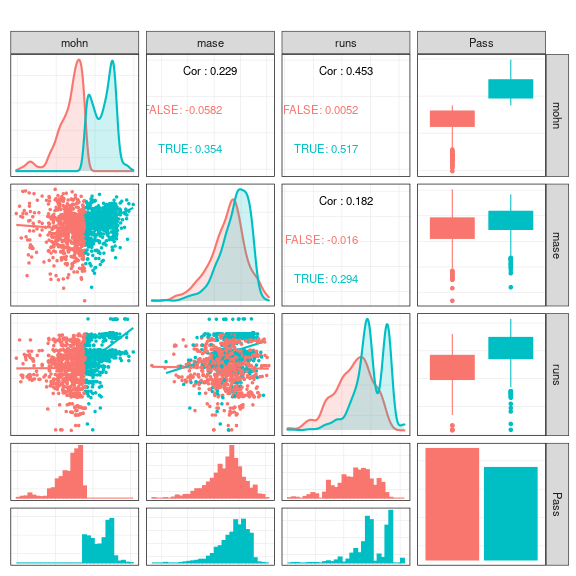
\includegraphics[width=0.75\textwidth]{figures/ggpair-1.png} \caption{Correlations between weighting diagnostics.}
\label{fig:wts}       
\end{figure}

\newpage
\begin{figure}[!ht]
	\centering
	\begin{subfigure}{0.9\textwidth}
		\centering
		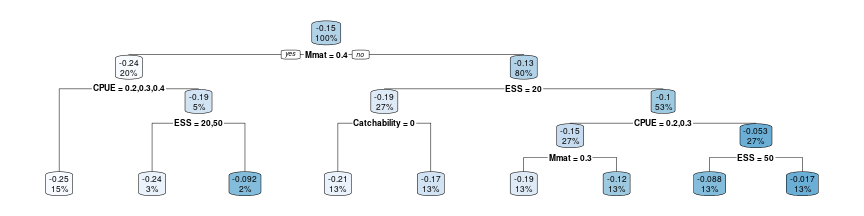
\includegraphics[width=\textwidth]{figures/a-tree-1.png}
		\caption{Regression Tree}
		\label{fig:tree}
	\end{subfigure}
	\hfill
	\begin{subfigure}{0.9\textwidth}  
		\centering 
		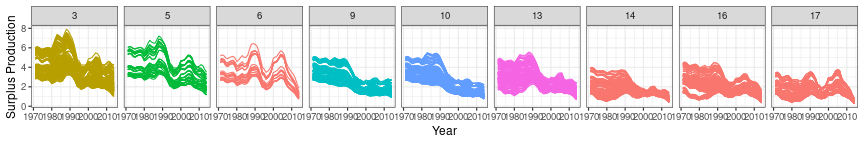
\includegraphics[width=\textwidth]{figures/a-tree-biomass-1.png}
		\caption{SSB}
		\label{fig:tree-b}
	\end{subfigure}
	\begin{subfigure}{0.9\textwidth}  
		\centering 
		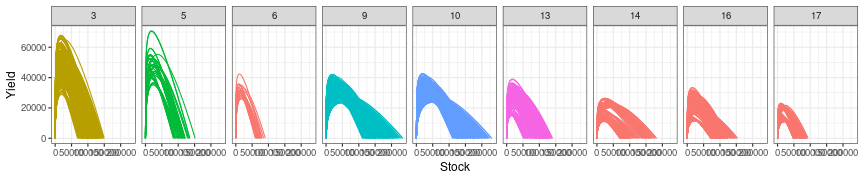
\includegraphics[width=\textwidth]{figures/a-tree-pf-1.png}
		\caption{Production Function}
		\label{fig:tree-pf}
	\end{subfigure}
	\begin{subfigure}{0.9\textwidth}
		\centering
	    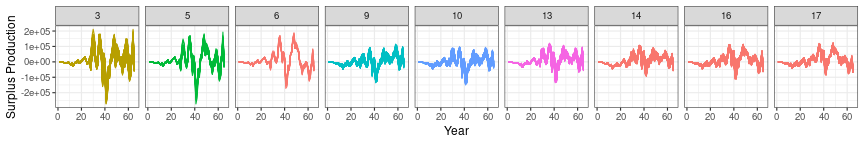
\includegraphics[width=\textwidth]{figures/a-tree-sp-1.png}
		\caption{Surplus Production}
		\label{fig:tree-sp}
	\end{subfigure}
	\caption{Mohn's $\rho$}
	\label{fig:tree}
\end{figure}


\begin{figure}
        \begin{subfigure}[b]{0.5\textwidth}
                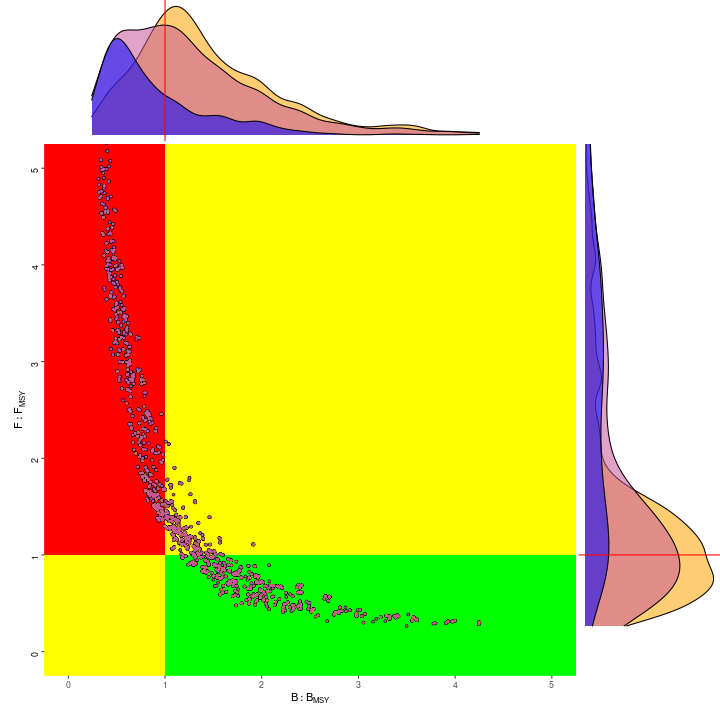
\includegraphics[width=\linewidth]{figures/kobe-mohn3-2.png}
                \caption{Kobe}
                \label{fig:kobe-wt}
        \end{subfigure}%
        \begin{subfigure}[b]{0.5\textwidth}
                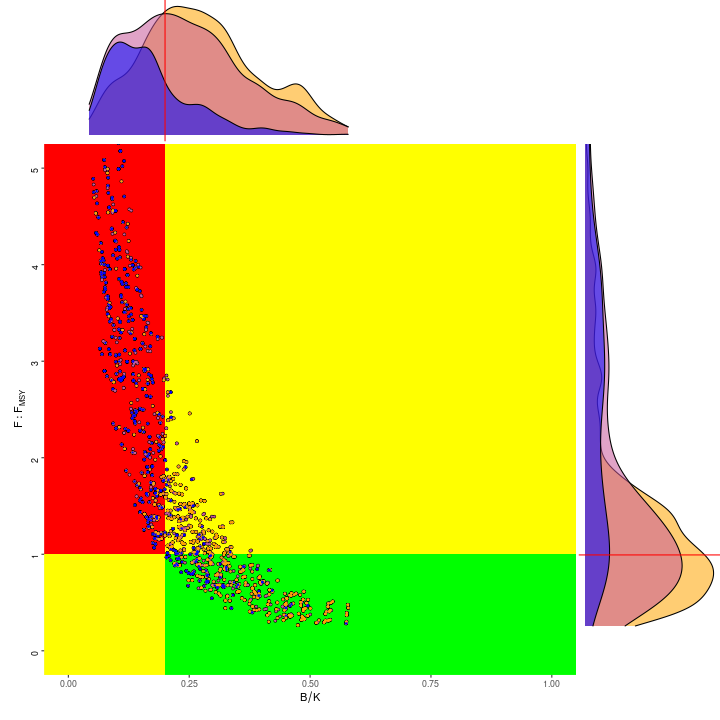
\includegraphics[width=\linewidth]{figures/majuro-mohn3-all-1.png}
                \caption{Majuro}
                \label{fig:majuro-wt}
        \end{subfigure}%
        \caption{Phase plots for all 1440 grid models, with equal, AIC, and skill weighting identifying models that pass the Mohn's $\rho$ test for hindcasts with 3 year ahead forecasts .}
        \label{fig:phase-wt}
\end{figure}


%\begin{figure}[ht!]\centering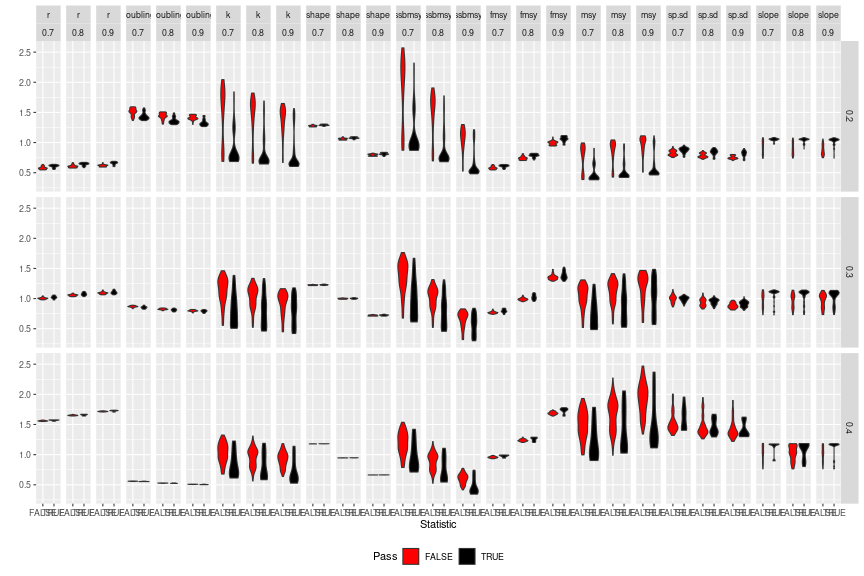
\includegraphics[width=1\textwidth]{figures/param-box-mohn3-1.png}\caption{Summary statistics, will re-do for $F/F_{MSY}$, $B/B_{MSY}$, $r$, $K$, $p$ and $sd(sp)$, and population doubling time.}\label{fig:smry}\end{figure}

\newpage
\begin{figure}[!ht]
	\centering
	\begin{subfigure}{0.32\textwidth}
		\centering
		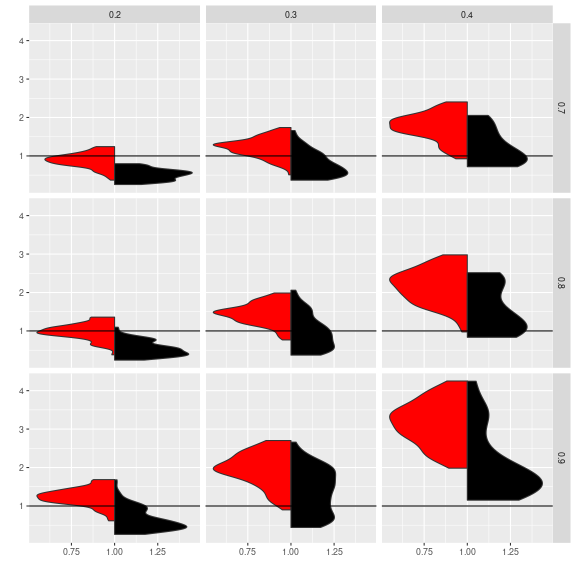
\includegraphics[width=\textwidth]{figures/v-b-1.png}
		\caption{$SSB/B_{MSY}$}
		\label{fig:grid-bmsy}
	\end{subfigure}
	\begin{subfigure}{0.32\textwidth}  
		\centering 
		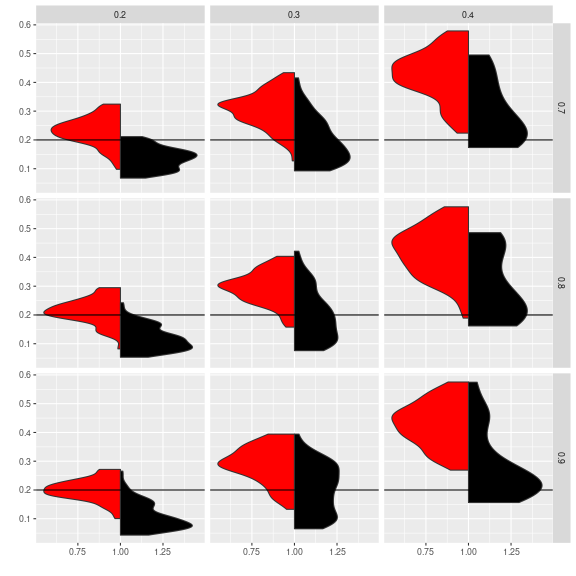
\includegraphics[width=\textwidth]{figures/v-m-1.png}
		\caption{$SSB/K$}
		\label{fig:grid-blim}
	\end{subfigure}
	\begin{subfigure}{0.32\textwidth}  
		\centering 
		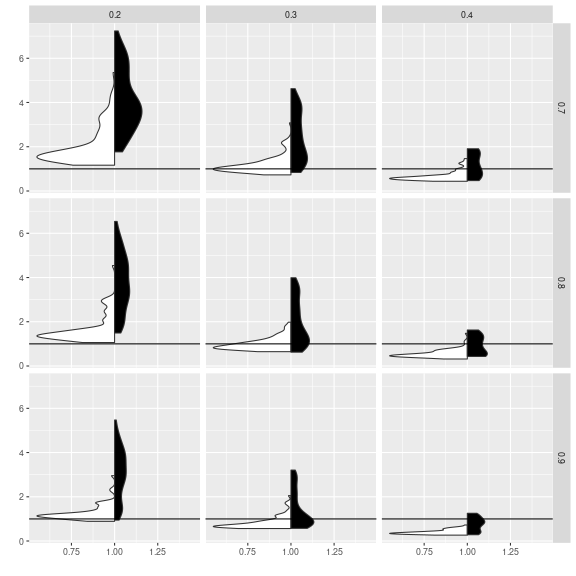
\includegraphics[width=\textwidth]{figures/v-h-1.png}
		\caption{$F/F_{MSY}$}
		\label{fig:grid-fmsy}
	\end{subfigure}
	\begin{subfigure}{0.32\textwidth}  
		\centering 
		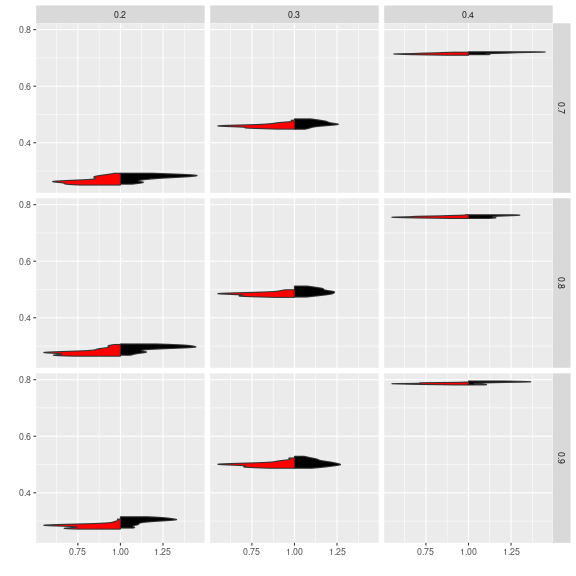
\includegraphics[width=\textwidth]{figures/v-r-1.png}
		\caption{$r$}
		\label{fig:grid-r}
	\end{subfigure}	\begin{subfigure}{0.32\textwidth}  
		\centering 
		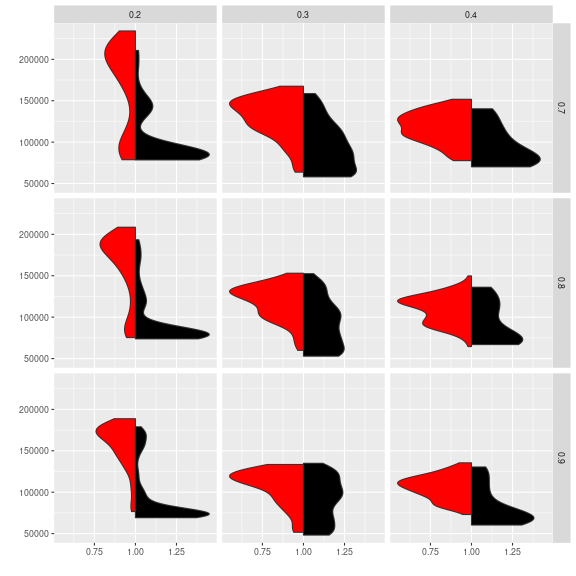
\includegraphics[width=\textwidth]{figures/v-k-1.png}
		\caption{$K$}
		\label{fig:grid-k}
	\end{subfigure}	\begin{subfigure}{0.32\textwidth}  
		\centering 
		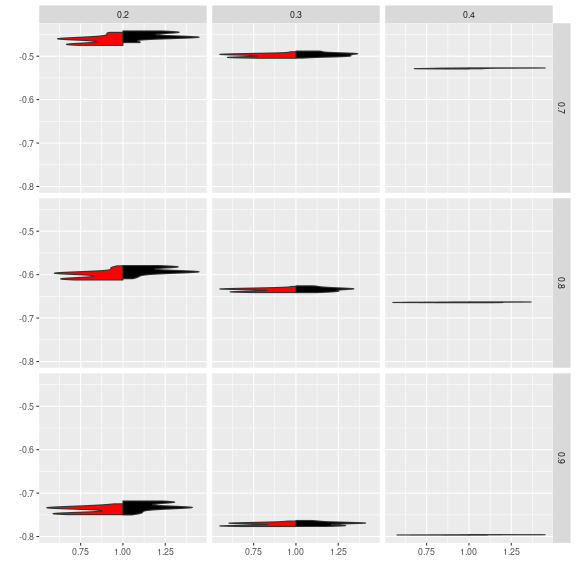
\includegraphics[width=\textwidth]{figures/v-p-1.png}
		\caption{$p$}
		\label{fig:grid-p}
	\end{subfigure}
	\begin{subfigure}{0.32\textwidth}  
		\centering 
		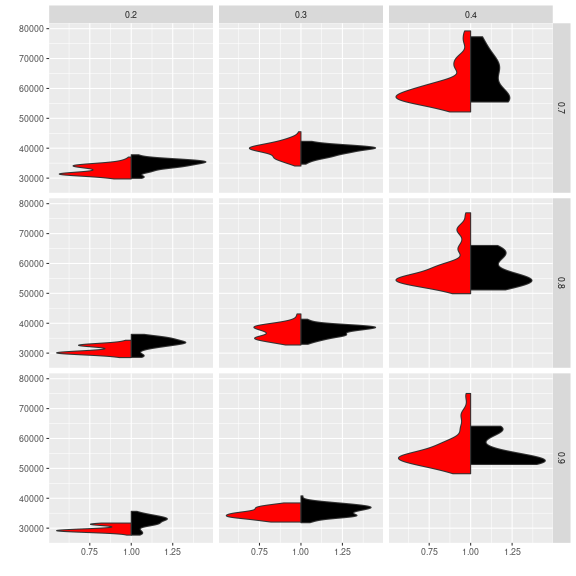
\includegraphics[width=\textwidth]{figures/v-sp-1.png}
		\caption{$sd(sp)$}
		\label{fig:grid-sp}
	\end{subfigure}	\begin{subfigure}{0.32\textwidth}  
		\centering 
		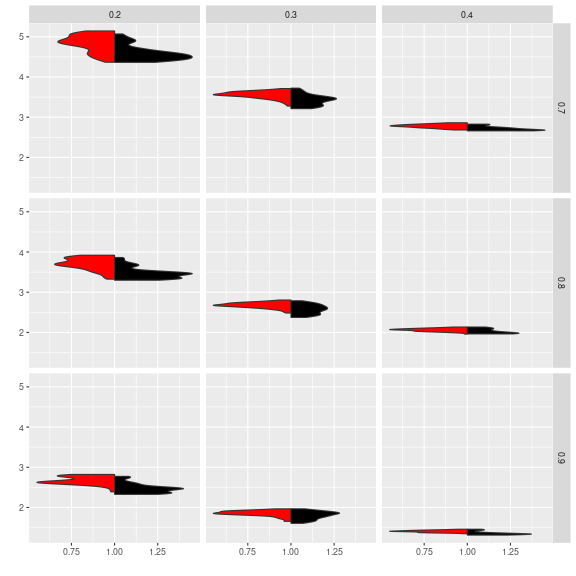
\includegraphics[width=\textwidth]{figures/v-d-1.png}
		\caption{Population doubling time}
		\label{fig:grid-dt}
	\end{subfigure}
	\caption{}
	\label{ref:grid}
\end{figure}

\iffalse
\begin{figure}[ht!]\centering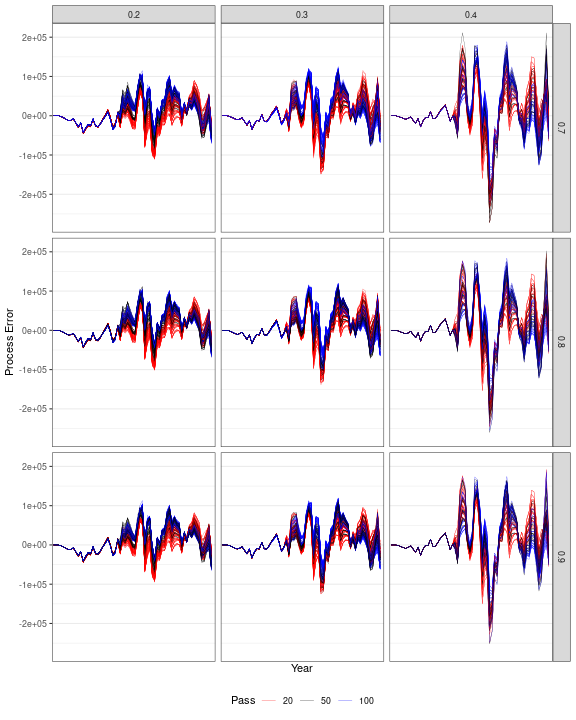
\includegraphics[width=0.75\textwidth]{figures/pf-1.png} 
\caption{Surplus Production by steepness and mature natural mortality}
\label{fig:sp}       
\end{figure}
\fi



\end{document}

\clearpage
\newpage
\section{Tables}

\begin{table}[!ht]
\label{tab:grid}
\caption{Operating Model Scenarios; Base Case values in bold.}  
\begin{center}
\label{tab:datasumm}
\begin{tabular}{|lccc|}
\hline
& {\tiny Levels (N)} & {\tiny $\prod$ N} & {\tiny Values} \\ %& {\tiny Prior} & {\tiny Weighting}\\
\hline\hline
{\tiny Natural mortality (M)& {\tiny 5}}  & {\tiny   5}  & {\tiny  0202  \textbf{0303} 0404 0403 0402}    \\
{\tiny Steepness of the stock-recruitment relationship}}& {\tiny 3} 	 & {\tiny 15}  & {\tiny  \textbf{.7}; 0.8; 0.9} \\
{\tiny Variability of recruitment (sigmaR)}& {\tiny 2} 	 & {\tiny  30}  & {\tiny  \textbf{0.4}; 0.6} \\
{\tiny Effective Sampling Size of the length composition data (ESS)}& {\tiny 3} & {\tiny  90}  & {\tiny  20; \textbf{50}; 100} \\
{\tiny CV for fit to CPUE (cpuecv)}& {\tiny 2} 	 & {\tiny  360}  & {\tiny  0.2;  \textbf{0.3}; 0.4; 0.5} \\
{\tiny Yearly increase in catchability coefficient of CPUE (llq)}& {\tiny 2} 	 & {\tiny   720}  & {\tiny  \textbf{0\%}; 0.25\%} \\
{\tiny Selectivity (llsel)}& {\tiny 2}}& {\tiny 1440}} & {\tiny  \textbf{logistic} double normal} \\
\hline

\end{tabular}
\end{center}
\end{table}

\begin{table}[!ht]
\caption{Mohn's $\rho$ for retrospective analysis.}  
\label{tab:retro}
\centering
\begin{tabular}{rllr}
  \hline
 & run & variable & $\rho$ \\ 
  \hline
  1 & ... & stock & ... \\ 
   \hline
\end{tabular}
\end{table}


\end{document}

\subsection{How to include Figures}

First you have to upload the image file from your computer using the upload link the project menu. Then use the includegraphics command to include it in your document. Use the figure environment and the caption command to add a number and a caption to your figure. See the code for Figure \ref{fig:frog} in this section for an example.

\subsection{How to add Comments}

Comments can be added to your project by clicking on the comment icon in the toolbar above. % * <john.hammersley@gmail.com> 2016-07-03T09:54:16.211Z:
%
% Here's an example comment!
%
To reply to a comment, simply click the reply button in the lower right corner of the comment, and you can close them when you're done.

Comments can also be added to the margins of the compiled PDF using the todo command\todo{Here's a comment in the margin!}, as shown in the example on the right. You can also add inline comments:

\todo[inline, color=green!40]{This is an inline comment.}

\subsection{How to add Tables}

Use the table and tabular commands for basic tables --- see Table~\ref{tab:widgets}, for example. 

\begin{table}
\centering
\begin{tabular}{l|r}
Item & Quantity \\\hline
Widgets & 42 \\
Gadgets & 13
\end{tabular}
\caption{\label{tab:widgets}An example table.}
\end{table}

\subsection{How to write Mathematics}

\LaTeX{} is great at typesetting mathematics. Let $X_1, X_2, \ldots, X_n$ be a sequence of independent and identically distributed random variables with $\text{E}[X_i] = \mu$ and $\text{Var}[X_i] = \sigma^2 < \infty$, and let
\[S_n = \frac{X_1 + X_2 + \cdots + X_n}{n}
      = \frac{1}{n}\sum_{i}^{n} X_i\]
denote their mean. Then as $n$ approaches infinity, the random variables $\sqrt{n}(S_n - \mu)$ converge in distribution to a normal $\mathcal{N}(0, \sigma^2)$.


\subsection{How to create Sections and Subsections}

Use section and subsections to organize your document. Simply use the section and subsection buttons in the toolbar to create them, and we'll handle all the formatting and numbering automatically.

\subsection{How to add Lists}

You can make lists with automatic numbering \dots

\begin{enumerate}
\item Like this,
\item and like this.
\end{enumerate}
\dots or bullet points \dots
\begin{itemize}
\item Like this,
\item and like this.
\end{itemize}

\subsection{How to add Citations and a References List}

You can upload a \verb|.bib| file containing your BibTeX entries, created with JabRef; or import your \href{https://www.overleaf.com/blog/184}{Mendeley}, CiteULike or Zotero library as a \verb|.bib| file. You can then cite entries from it, like this: \cite{greenwade93}. Just remember to specify a bibliography style, as well as the filename of the \verb|.bib|.

You can find a \href{https://www.overleaf.com/help/97-how-to-include-a-bibliography-using-bibtex}{video tutorial here} to learn more about BibTeX.

We hope you find Overleaf useful, and please let us know if you have any feedback using the help menu above --- or use the contact form at \url{https://www.overleaf.com/contact}!
